\documentclass{article}
\usepackage[top=3cm, bottom=3cm, left = 2cm, right = 2cm]{geometry}
\geometry{a4paper}
\usepackage[T1]{polski}
\usepackage[utf8]{inputenc}
\usepackage{titling}
\usepackage{caption}
\usepackage[parfill]{parskip}
\usepackage{hyperref}
\usepackage{multirow}
\usepackage{graphicx}
\usepackage{tikz}
\usetikzlibrary{decorations.markings}
\usepackage{subcaption}
\usepackage{pgffor}

\author{Jakub Jaśków}
\title{Algorytmy Metaheurustyczne - Lista nr 1}
\begin{document}
\maketitle
\section*{Cel}
Celem zadania jest sprawdzenie skuteczności heurystyki Local Search na przykładzie euklidesowego problemu komiwojażera oraz
zbadanie wpływu wyboru rozwiązania początkowego i metody generowania otoczenia na jakość rozwiązania.

\section*{Local Search}
\subsection*{Invert}
Otoczeniem rozwiązania reprezentowanego przez permutację $\pi$ jest zbiór rozwiązań uzyskanych przy użyciu pojedynczego 
ruchu $invert(\pi, i, j)$, który zamienia kolejność wierzchołków od $i$-tego do $j$-tego.

\subsubsection*{Własność invert}
Invert "rozplątuje" pętle w cyklu. Pętle takie są nieoptymalne.
\begin{figure}[h!]
    \centering
    \begin{subfigure}{0.5\textwidth}
        \centering
        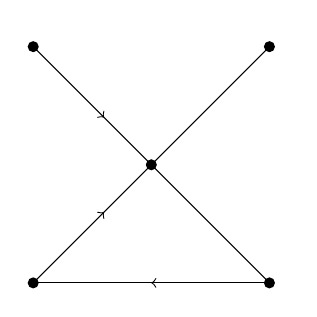
\begin{tikzpicture}
            \coordinate (A) at (0,3);
            \coordinate (B) at (3,3);
            \coordinate (C) at (3,0);
            \coordinate (D) at (0,0);
            \coordinate (P) at (1.5, 1.5);
        
            \fill (A) circle (2pt) node[above right] {};
            \fill (B) circle (2pt) node[above right] {};
            \fill (C) circle (2pt) node[above right] {};
            \fill (D) circle (2pt) node[above right] {};
            \fill (P) circle (2pt) node[above right] {};

            \draw[postaction={decorate,decoration={markings,mark=at position 0.3 with {\arrow{>}}}}] (A) -- (C);
            \draw[postaction={decorate,decoration={markings,mark=at position 0.5 with {\arrow{>}}}}] (C) -- (D);
            \draw[postaction={decorate,decoration={markings,mark=at position 0.3 with {\arrow{>}}}}] (D) -- (B);
            %\draw[postaction={decorate,decoration={markings,mark=at position 0.5 with {\arrow{>}}}}] (B) -- (A);
        
        \end{tikzpicture}
    \end{subfigure}%
    \begin{subfigure}{0.5\textwidth}
        \centering
        \begin{tikzpicture}
            \coordinate (A) at (0,3);
            \coordinate (B) at (3,3);
            \coordinate (C) at (3,0);
            \coordinate (D) at (0,0);
        
            \fill (A) circle (2pt) node[above right] {};
            \fill (B) circle (2pt) node[above right] {};
            \fill (C) circle (2pt) node[above right] {};
            \fill (D) circle (2pt) node[above right] {};

            %\draw[postaction={decorate,decoration={markings,mark=at position 0.5 with {\arrow{>}}}}] (A) -- (B);
            \draw[postaction={decorate,decoration={markings,mark=at position 0.5 with {\arrow{>}}}}] (B) -- (C);
            \draw[postaction={decorate,decoration={markings,mark=at position 0.5 with {\arrow{>}}}}] (C) -- (D);
            \draw[postaction={decorate,decoration={markings,mark=at position 0.5 with {\arrow{>}}}}] (D) -- (A);
            
        \end{tikzpicture}
    \end{subfigure}
\end{figure}
\subsection*{Wybór rozwiązania początkowego}
\begin{enumerate}
    \item rozwiązanie zbudowane na podstawie MST
    \item rozwiązanie wygenerowane w sposób losowy
\end{enumerate}

\subsection*{Przegląd sąsiedztwa}
\begin{enumerate}
    \item przeglądanie całego sąsiedztwa(rozmiar: $O(n^2)$)
    \item przeglądanie $n$ losowo wybranych sąsiadów(rozmiar: $O(n)$)
\end{enumerate}

\subsection*{Generowanie najlepszego kandydata}
Gdy rozwiązaniem początkowym jest rozwiązanie generowane na podstawie MST to $\sqrt{n}$ razy 
generujemy takie rozwiązanie zaczynając od losowego wierzchołka drzewa a następnie 
używamy go jako startowego w algorytmie Local Search. \newline
Gdy rozwiązaniem początkowym jest rozwiązanie losowe to $n$ razy powtarzamy losowanie rozwiązania 
oraz poprawianie go algorytmem Local Search. W przypadku $n > 1000$ procedurę powtarzamy tylko 100 razy.

W każdym przypadku jako wynik wybieramy rozwiązanie o najmniejszej wadze.

\section*{Wyniki}
Oznaczenia metod generujących kandydatów:
\begin{itemize}
    \item LS1 - algorytm Local Search startujący z rozwiązania wygenerowane z losowego wierzchołka MST i przeglądający całe otoczenie w każdej iteracji
    \item LS2 - algorytm Local Search startujący z losowego rozwiązania i przeglądający całe otoczenie w każdej iteracji
    \item LS3 - algorytm Local Search startujący z losowego rozwiązania i przeglądający $n$ losowych sąsiadów w każdej iteracji
\end{itemize}
\begin{table}[h!]
    \centering
    \begin{tabular}{|c|c|c|c|c|c|}
        \hline
        \multirow{3}{*}{Przykład} & Suma wag & Suma wag & Suma wag & Suma wag  & Suma wag  \\
        & rozwiązania  & kandydata & najlepszego & najlepszego & najlepszego \\
        & optymalnego & opartego o MST & rozwiązania LS1 & rozwiązania LS2  & rozwiązania LS3 \\
        \hline
        xqf131 & 564 & 718 & 596 & 578 & 880 \\
        \hline
        xqg237 & 1019 & 1445 & 1067 & 1062 & 1676 \\
        \hline
        pma343 & 1368 & 1883 & 1436 & 1424 & 2312 \\
        \hline
        pka379 & 1332 & 1855 & 1398 & 1399 & 2271 \\
        \hline
        bcl380 & 1621 & 2319 & 1711 & 1728 & 3095 \\
        \hline
        pbl395 & 1281 & 1871 & 1351 & 1359 & 2390 \\
        \hline
        pbk411 & 1343 & 1935 & 1421 & 1426 & 2521 \\
        \hline
        pbn423 & 1365 & 1918 & 1453 & 1454 & 2473 \\
        \hline
        pbm436 & 1443 & 2119 & 1532 & 1535 & 2685 \\
        \hline
        xql662 & 2513 & 3691 & 2661 & 2707 & 4926 \\
        \hline
        xit1083 & 3558 & 5190 & 3803 & 3919 & 7256 \\
        \hline
        icw1483 & 4416 & 6754 & 4757 & 4839 & 9293 \\
        \hline
        djc1785 & 6115 & 8908 & 6477 & 6697 & 12617 \\
        \hline
        dcb2086 & 6600 & 9777 & 7107 & 7313 & 14780 \\
        \hline
        pds2566 & 7643 & 11427 & 8182 & 8506 & 17506 \\
        \hline
    \end{tabular}
    % \caption{Porównanie metod generowania kandydatów dla problemu komiwojażera.}
\end{table}

\begin{table}[h!]
    \centering
    \begin{tabular}{|c|c|c|c|c|c|c|c|c|c|}
        \hline
        \multirow{3}{*}{Przykład} & \multicolumn{3}{|c|}{Rozwiązania LS1} & \multicolumn{3}{|c|}{Rozwiązania LS2}  & \multicolumn{3}{|c|}{Rozwiązania LS3}  \\
        \cline{2-10}
        & liczba & \multicolumn{2}{c|}{suma wag} & liczba & \multicolumn{2}{c|}{suma wag} & liczba & \multicolumn{2}{c|}{suma wag} \\
        \cline{3-4} \cline{6-7} \cline{9-10}
        & popraw & średnia & minimum & popraw & średnia & minimum & popraw & średnia & minimum \\
        \hline
        xqf131 & 28.8 & 601.9 & 596 & 133.3 & 612.4 & 578 & 111.9 & 1044.4 &  880 \\
        \hline
        xqg237 & 37.0 & 1083.7 & 1067 & 260.5 & 1115.8 & 1062 & 225.2 & 2090.4 &  1676 \\
        \hline
        pma343 & 75.8 & 1450.3 & 1436 & 403.5 & 1484.7 & 1424 & 366.3 & 2835.0 &  2312 \\
        \hline
        pka379 & 78.9 & 1416.3 & 1398 & 448.7 & 1445.9 & 1399 & 408.9 & 2769.7 &  2271 \\
        \hline
        bcl380 & 62.7 & 1749.3 & 1711 & 446.7 & 1817.5 & 1728 & 374.2 & 3827.0 &  3095 \\
        \hline
        pbl395 & 80.0 & 1371.5 & 1351 & 458.8 & 1429.0 & 1359 & 387.4 & 2952.4 &  2390 \\
        \hline
        pbk411 & 81.6 & 1437.9 & 1412 & 483.7 & 1488.5 & 1426 & 406.6 & 3162.3 &  2512 \\
        \hline
        pbn423 & 72.3 & 1473.9 & 1453 & 497.0 & 1521.6 & 1454 & 419.8 & 3200.2 & 2473 \\
        \hline
        pbm436 & 97.85 & 1562.5 & 1543 & 512.8 & 1612.0 & 1535 & 433.4 & 3363.1 & 2685 \\
        \hline
        xql662 & 122.6 & 2690.4 & 2661 & 811.4 & 2813.3 & 2707 & 697.2 & 6035.1 & 4926 \\
        \hline
        xit1083 & 191.6 & 3847.2 & 3803 & 1383.7 & 4021.2 & 3919 & 1212.0 & 9052.2 & 7256 \\
        \hline
        icw1483 & 278.8 & 4809.8 & 4757 & 1929.4 & 4990.5 & 4839 & 1695.5 & 11436.9 & 9293 \\
        \hline
        djc1785 & 382.6 & 6533.8 & 6477 & 2348.9 & 6872.1 & 6697 & 2065.4 & 15529.9 & 12617 \\
        \hline
        dcb2086 & 390.9 & 7154.2 & 7107 & 2796.6 & 7457.8 & 7313 & 2457.2 & 17776.7 & 7107 \\
        \hline
        pds2566 & 457.3 & 8271.4 & 8182 & 3485.9 & 8701.8 & 8506 & 3052.0 & 21375.1 & 17506 \\
        \hline
    \end{tabular}
    \caption{Podsumowanie działania Local Search dla problemu komiwojażera.}
\end{table}

\section*{Grafy}
\def \myArray{xqf131, xqg237, pma343, pka379, bcl380, pbl395, pbk411, pbn423, pbm436, xql662, xit1083, icw1483, djc1785, dcb2086, pds2566}

\foreach \text in \myArray {
    \subsection{\text}

    \begin{figure}[h!]
        \centering
        \includegraphics[height=5.0cm]{../../plots/\text-ls-imp.png}
    \end{figure}
    
    \begin{figure}[h!]
        \centering
        \includegraphics[height=5.0cm]{../../plots/\text-tsp-mst.png}
    \end{figure}

    \begin{figure}[h!]
        \centering
        \includegraphics[height=5.0cm]{../../plots/\text-tsp-ls-mst.png}
    \end{figure}

    \begin{figure}[h!]
        \centering
        \includegraphics[height=5.0cm]{../../plots/\text-tsp-ls-mst-stats.png}
    \end{figure}

    \newpage

    \begin{figure}[h!]
        \centering
        \includegraphics[height=5.0cm]{../../plots/\text-tsp-ls-rand.png}
    \end{figure}

    \begin{figure}[h!]
        \centering
        \includegraphics[height=5.0cm]{../../plots/\text-tsp-ls-rand-stats.png}
    \end{figure}

    \begin{figure}[h!]
        \centering
        \includegraphics[height=5.0cm]{../../plots/\text-tsp-ls-rand-rand.png}
    \end{figure}

    \begin{figure}[h!]
        \centering
        \includegraphics[height=5.0cm]{../../plots/\text-tsp-ls-rand-rand-stats.png}
    \end{figure}

    \newpage
}

\end{document}
